\section{RNG\_\-UNIFORM Class Reference}
\label{classRNG__UNIFORM}\index{RNG_UNIFORM@{RNG\_\-UNIFORM}}
{\tt \#include $<$rng\_\-uniform.h$>$}

Inheritance diagram for RNG\_\-UNIFORM::\begin{figure}[H]
\begin{center}
\leavevmode
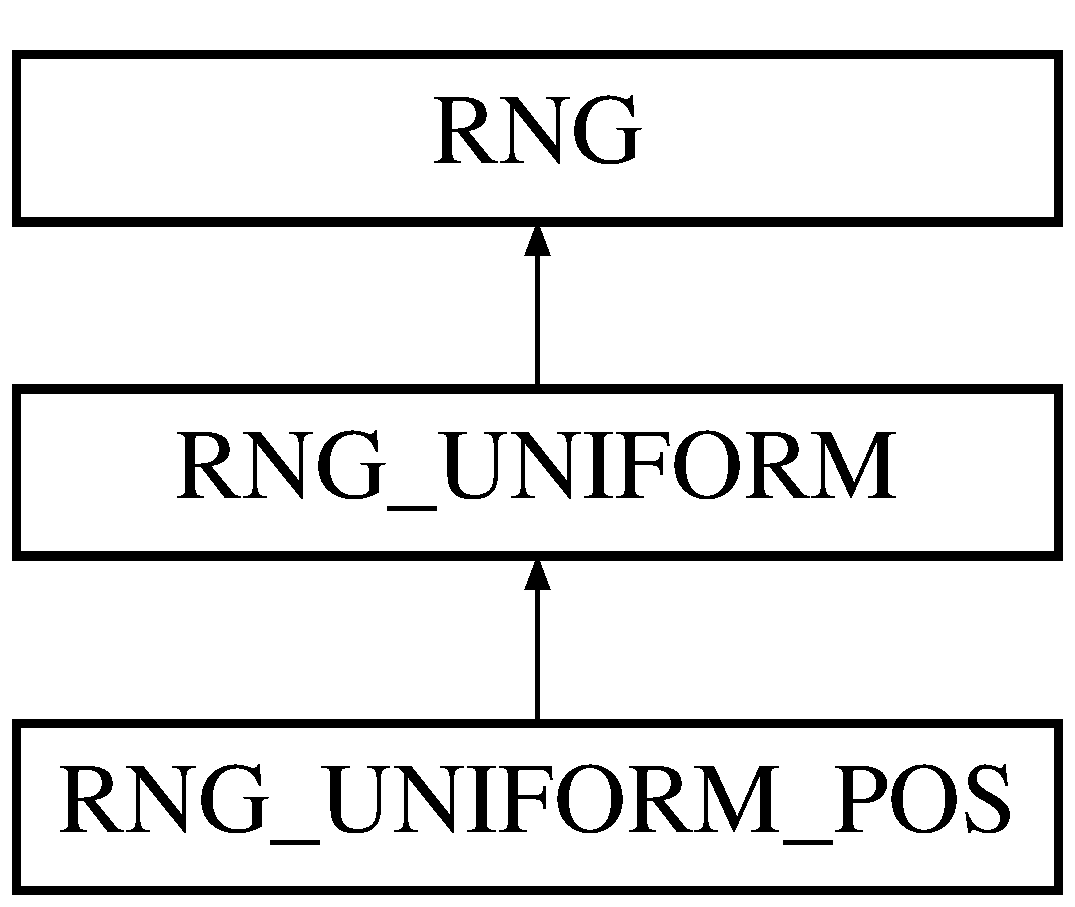
\includegraphics[height=3cm]{classRNG__UNIFORM}
\end{center}
\end{figure}
\subsection*{Public Member Functions}
\begin{CompactItemize}
\item 
\textbf{RNG\_\-UNIFORM} (const gsl\_\-rng\_\-type $\ast$)\label{classRNG__UNIFORM_7b87b63759759c2ceaeb5c66544d60b2}

\item 
\textbf{RNG\_\-UNIFORM} (const gsl\_\-rng\_\-type $\ast$, const unsigned long)\label{classRNG__UNIFORM_b74facd380f0729c381199534f5056f4}

\item 
virtual long double \textbf{Get} ()\label{classRNG__UNIFORM_6ce3b4be6c400c9f753914605f129ce3}

\end{CompactItemize}


\subsection{Detailed Description}
\begin{Desc}
\item[Author:]Krishnan S \end{Desc}




The documentation for this class was generated from the following files:\begin{CompactItemize}
\item 
rng\_\-uniform.h\item 
rng\_\-uniform.cpp\end{CompactItemize}
